
\subsection{Second level functions} \label{sec:2ndlvl}

	\subsubsection{Biological component: \texttt{biols.om}}
	
	The call to the function within \texttt{FLBEIA} is done as:
	
	\begin{center}
		\texttt{biols.om(biols, fleets, SRs, BDs, covars, biols.ctrl, year, season)}
	\end{center}
		
		This function projects the stocks one season forward. The projection is done independently stock by stock by the third level function specified for each stock in \texttt{biols.ctrl} object. Currently, there are three population dynamics functions implemented, one corresponding to age structured populations, \texttt{ASPG}, the second one to biomass dynamics populations, \texttt{BDPG} and another one to fixed populations (given as input), \texttt{fixedPopulation}. These functions do not include predation among stocks, but this kind of models could be implemented and used in the algorithm if necessary.

  \noindent Control arguments:
  \begin{description}
    \item[\texttt{biols.control}:] This argument is a list which contains the necessary information to run the third level functions that are called by \texttt{biols.om}. The elements depend on the third and lower level functions used to describe the 	dynamics of the stocks. The list must contain at least one element per stock and the name of the element must coincide exactly with the name used in $\texttt{biols}$ argument so it can be used to link the population with its dynamics model. At the same time, each of these elements must be a list with at least one element, \texttt{growth.model}, which specifies the name of the function used to describe population dynamics (options: \texttt{ASPG}, \texttt{BDPG} or \texttt{fixedPopulation}).
    
  	For example:
       
    \begin{Schunk}
      \begin{Sinput}
        > biols.ctrl
      \end{Sinput}
      
      \begin{Soutput}
        $NHKE
        $NHKE$growth.model
        [1] "ASPG"
        
        $CMON
        $CMON$growth.model
        [1] "BDPG"
        
        $FAKE
        $FAKE$growth.model
        [1] "ASPG"
      \end{Soutput}
    \end{Schunk}
  \end{description}

	
	\subsubsection{Fleets component: \texttt{fleets.om}}
		
		The call to \texttt{fleets.om} function within \texttt{FLBEIA} is done as:
		
		\begin{center}
			\texttt{fleets.om(fleets, biols, covars, advice, fleets.ctrl, advice.ctrl, year, season) }
		\end{center}

	This function projects the fleets one season forward. 
 	The main argument, \texttt{fleets}, is an object of class \texttt{FLFleetsExt} (for more detail see Section~\ref{sec:1stlvl})
  %, an extension of the \texttt{FLFleet} object. The difference is in the \texttt{catches} slot that in the case of 
	%\texttt{FLFleetsExt} object is of class \texttt{FLCatchesExt}.  \texttt{FLCatchExt} objects 
	% are equal to the original \texttt{FLCatch} but has 2 extra slots, \texttt{alpha} and
	%\texttt{beta}. These two slots have been added to store Cobb-Douglas production function parameters.
	
	The function is divided in three processes related to fleet dynamics: the effort model, the price model and the capital model.
	Effort and capital models are fleet specific, whereas price model is fleet and stock specific.
	First, \texttt{fleets.om} calls the effort model and it updates the slots related to 
	effort and catch. The effort models are called independently fleet by fleet. Then, \texttt{fleets.om}
	calls the price model in fleet by fleet and stock by stock basis, which updates the \texttt{price} slot
	in the \texttt{fleets} object. Finally, but only in the last season of the year, the function calls the capital model. 
  Thus, investment and disinvestment is only done annually. 
	The capital model is called independently fleet by fleet. 
	
\begin{description}
	\item[Effort model:] This part of the model simulates the tactical behaviour of the fleet every season and iteration.
	 In each time step and iteration, the effort exerted by each individual fleet and its effort-share among metiers is 
	 calculated depending on the stock abundance, management restrictions or others. 
	 After that, the catch produced by the combination of effort and effort-share
	 is calculated and \texttt{discards, discards.n, landings, landings.n} slots are filled.
	 Other stored variables in \texttt{fleets.ctrl} could also be updated here, for example \texttt{quota.share},
	 as a result of the exerted effort. 
	 
	 The effort model is specified at fleet level, so each fleet can follow a different effort model.
	 At the moment there are 4 functions available: \texttt{fixedEffort, SMFB, SSFB} and \texttt{MaxProfit}. 
	 To write new functions for effort, it must be taken into account that the input arguments 
	 must be found among \texttt{fleets.om} function arguments and that the output must be a 
	 list with updated \texttt{FLFleetsExt} and \texttt{fleets.ctrl} objects, i.e.:
				
  \begin{Schunk}
    \begin{Sinput}
    list(fleets = my_fleets_obj, fleets.ctrl = my_fleets.ctrl_obj)
    \end{Sinput}
  \end{Schunk}	 	
		
			 	  
	\item[Price Model:] The price model updates the price-at-age at stock, metier and fleet level in each time
	step and iteration. 
	
	At the moment, there are 2 functions available: 
	\texttt{fixedPrice} and \texttt{elasticPrice}. 
	To write new functions for price it must be taken into account that the input arguments 
	must be found among \texttt{fleets.om} function arguments and that the output must be a 
	list with an updated \texttt{FLFleetsExt} object.
				
	\item[Capital Model:] This module is intended to simulate the strategic behaviour of the fleets, namely, the investment and disinvestment dynamics. 
	The model is applied at fleet level and in an annual basis and can affect fleets'  
	capacity and  catchability. Catchability could be modified through investment in technological improvement 
	and capacity as a result of an increase (investment) or decrease (disinvestment) in the number of vessels.  
	Changes in fleets' capacities could produce a variation in quota share among fleets, for example.
	Thus, the corresponding change would have to be done in \texttt{fleets.ctrl} object. 
	
	At the moment, there are 2 functions available: \texttt{fixedCapital} and \texttt{SCD}.
	To write new functions for capital dynamics, as for effort and price, it must be taken into account 
	that the input arguments must be found among \texttt{fleets.om} function arguments and that the 
	output must be a list with updated \texttt{FLFleetsExt} and \texttt{fleets.ctrl} objects.				
\end{description}


\noindent Control arguments:
\begin{description}
  \item[\texttt{fleets.ctrl}:] The most simple example of fleet dynamics model and hence 
  	the most simple \texttt{fleets.ctrl} object correspond with the model where all the parameters 
		in \texttt{fleets} object are given as input and maintained fixed
		 within the simulation. This is obtained using the third level functions, \texttt{fixedEffort, fixedPrice} and
		 \texttt{fixedCapital} which do not need any extra arguments. In the case of two fleets,
		 \texttt{FL1} and \texttt{FL2}, where \texttt{FL1} catches 3 stocks, \texttt{ST1, ST2} and \texttt{ST3} and \texttt{FL2}
		 catches  \texttt{ST1} and \texttt{ST3} stocks, the \texttt{fleets.ctrl} could be created using the following code:
     
  \begin{Schunk}
    \begin{Sinput}
    >fleets.ctrl <- list()
    
    # The fleets
    >fleets.ctrl[['FL1']] <- list()
    >fleets.ctrl[['FL2']] <- list()
    
    # Effort model per fleet.
    >fleets.ctrl[['FL1']]$effort.model <- 'fixedEffort'
    >fleets.ctrl[['FL2']]$effort.model <- 'fixedEffort'
    
    # Price model per fleet and stock.
    >fleets.ctrl[['FL1']][['ST1']]$price.model  <- 'fixedPrice'
    >fleets.ctrl[['FL1']][['ST2']]$price.model  <- 'fixedPrice'
    >fleets.ctrl[['FL1']][['ST3']]$price.model  <- 'fixedPrice'
    
    >fleets.ctrl[['FL2']][['ST1']]$price.model  <- 'fixedPrice'
    >fleets.ctrl[['FL2']][['ST3']]$price.model  <- 'fixedPrice'
    
    # Capital model by fleet.
    >fleets.ctrl[['FL1']]$capital.model  <- 'fixedCapital'
    >fleets.ctrl[['FL2']]$capital.model  <- 'fixedCapital'
    
    > fleets.ctrl
    \end{Sinput}
    \begin{Soutput}
      $FL1
      $FL1$effort.model
      [1] "fixedEffort"
      
      $FL1$ST1
      $FL1$ST1$price.model
      [1] "fixedPrice"
      
      $FL1$ST2
      $FL1$ST2$price.model
      [1] "fixedPrice"
      
      $FL1$ST3
      $FL1$ST3$price.model
      [1] "fixedPrice"
      
      $FL1$capital.model
      [1] "fixedCapital"
       
      $FL2
      $FL2$effort.model
      [1] "fixedEffort"
      
      $FL2$ST1
      $FL2$ST1$price.model
      [1] "fixedPrice"
      
      $FL2$ST3
      $FL2$ST3$price.model
      [1] "fixedPrice"
      
      $FL2$capital.model
      [1] "fixedCapital
    \end{Soutput}
  \end{Schunk}
\end{description}

 
	\subsubsection{Covariates component: \texttt{covars.om}}
	
	\texttt{covars.om} projects \texttt{covars} object one season forward.  
	\texttt{covars} object is a named list and the class and dimension of each element will depend 
	on the function used to project it into the simulation. 
	
	\noindent The call to \texttt{covars.om} function within \texttt{FLBEIA} is done as:

  \begin{center}
    \texttt{covars.om(biols, fleets, covars, advice, covars.ctrl, year, season) }
  \end{center}

	Internally, for each element in the \texttt{covars} list, it calls to the third level functions
	specified in the \texttt{covars.ctrl} object. At the moment, there exist 2 third level functions: \texttt{fixedCovar}, 
	which is used to work with variables that are input parameters not updated within the simulation and \texttt{ssb.get}, 
  which is used to get the real Spawning Stock Biomass of one of the simulated stocks. 
	
	The economic variables used in the capital dynamics model \texttt{SCD} should be stored in 
\texttt{covars} object and updated in each step using values in \texttt{fleets} object.

\noindent Control arguments:
\begin{description}
  \item[\texttt{covars.ctrl}:] This argument is a named list with one element per covariate and the names of the list must match those used 
  to name the \texttt{covars} object. Each of the elements is, at the same time, a list with, at least, one element, \texttt{dyn.model}, 
	which defines the dynamics of the covariate in question (options: \texttt{fixedCovar}, \texttt{ssb.get}).
\end{description}

	This way of working could be useful, for example, for environmental variables such as 
	sea surface temperature that could affect catchability or recruitment in the fleet and 
	biological operating models respectively and that are external to fishery system. 
	
	A covariate with a non-trivial 
	dynamics could be the abundance of certain animal which is not commercially exploited by the fleet, but which abundance
	affects the natural mortality of any of the exploited stocks. In this case, 2 extra functions will be needed, the function
	that defines the dynamics of the covariate and the function that models the natural mortality of the stock as a function of the abundance
	of the animal. The first function should be declared in \texttt{covars.ctrl} argument and the former one in 
	\texttt{biols.ctrl} argument as a stock dynamics model. 
 
	
	\subsubsection{Observation component: \texttt{observation.mp}}
	
	The observation component generates the necessary data to run the assessment models.
	The main function is \texttt{observation.mp} and it calls third level functions 
	which generate 3 possible objects, a \texttt{FLStock}, a \texttt{FLIndices} or a 
	\texttt{FLFleetsExt} object. The \texttt{FLStock} and  \texttt{FLIndices} objects
	are generated independently for each stock and the \texttt{FLFleetsExt} object
	jointly for all the fleets.
	
	\noindent The call to \texttt{observation.mp} function within \texttt{FLBEIA} is done, stock by stock, as follows:
	
  \begin{center}
  	\texttt{observation.mp(biols, fleets, covars, indices, advice, obs.ctrl, year, season, stknm) }
  \end{center}

  \noindent where \texttt{stknm} is the name of the stock to be observed and its name matches with those used in the \texttt{biols} object.
  
	The output of \texttt{observation.mp} is a list with 3 elements. The first element, \texttt{stock} is an object 
	of class \texttt{FLStock} or \texttt{NULL}, if a \texttt{FLStock} is not needed to run the assessment.
	The second element, \texttt{indices}, is a named list with one element per stock and its names correspond with those used 
	in \texttt{biols} object. The elements of the \texttt{indices} list are   
	of class  \texttt{FLIndices} or \texttt{NULL}, if a \texttt{FLIndices} is not needed to run the assessment.    
	The third element, \texttt{fleets.obs}, is an observed version of the original \texttt{fleets} object.
	At the moment, there is no third level function implemented to generate observed fleets.
  %The segmentation of the fleet in the observed version would be different to the real one.

% +++++ SONIA: NECESARIO REPASAR Y CORREGIR SIGUIENTE PARRAFO (se espera actualizacion por necesidades para anchoa) +++++

	As the management process is currently run in a yearly basis, the \texttt{unit} and \texttt{season}
	dimensions are collapsed in all the observed objects. Moreover, if the management process is being conducted at the end of year \texttt{y} the observed objects extend up to year \texttt{y-1}, 
  whereas they extend up to year \texttt{y} in the cases when management process is conducted in any other season as it happens in reality.
		
\noindent Control arguments:
\begin{description}
  \item[\texttt{obs.ctrl}:] %This argument is a list with one element per stock. If fleets were observed 
  	%the object should have also one element per fleet but as at the moment there are no functions that provide
		%observed version of \texttt{FLFleetsExt} object this option is not described here.
		The \texttt{obs.ctrl} object must be a named list where the names used correspond with 
		those used in the \texttt{FLBiols} object. Each stock element is, at the same time, a list 
		with two elements (\texttt{stkObs} and \texttt{indObs}) and these two elements are once again lists. 
		A scheme of \texttt{obs.ctrl} object is presented in Table~\ref{tb:A3.table5}.

    \begin{figure}[ht]
      \caption{obs.ctrl object scheme}
      \label{fig:obs.ctrl}
      \centering
        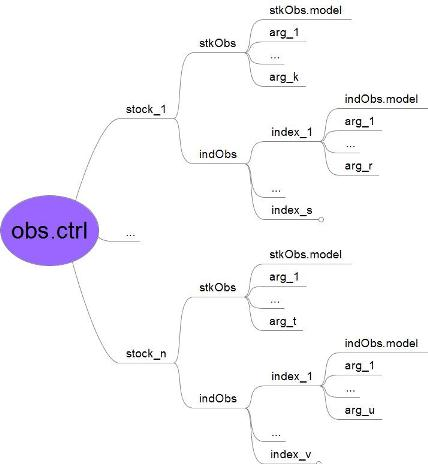
\includegraphics[width= 0.50 \textwidth]{obs_ctrl}
    \end{figure}

  	The \texttt{stkObs} element is a list with the arguments necessary to run the 
		third level function used to generate the \texttt{FLStock} object. In the list there must be 
		at least one element, \texttt{stkObs.model}, with the name of the third level function 
		that will be used two generate the \texttt{FLStock} object. If it is not required to generate a \texttt{FLStock} 
		object, then \texttt{NoObsStock} value should be assigned to \texttt{stkObs.model} argument and 
		this function will return the \texttt{NULL} object.

		The \texttt{indObs} element is a list with one element per index in the \texttt{FLIndices} object.
		Each element of the list is, at the same time, a list with the arguments necessary to run the 
		third level function used to generate the \texttt{FLIndex} object. In the list there must be 
		at least one element, \texttt{indObs.model}, with the name of the third level function 
		that will be used two generate the \texttt{FLIndex} object. If it is not required to generate a \texttt{FLIndices} 
		object, then \texttt{indObs} element will be set equal to \texttt{NoObsIndex} instead of a list and this will return 
		the \texttt{NULL} object instead of a \texttt{FLIndices} for the corresponding stock.

\end{description}


	\subsubsection{Assessment component: \texttt{assessment.mp}}
	
	The assessment component applies an existing assessment model to the stock data objects generated by the observation model 
	(\texttt{FLStock} and \texttt{FLIndices}). The assessment models are applied stock by stock, independently.
	
	\noindent The call to \texttt{assessment.mp} function within \texttt{FLBEIA} is done as follows:
	
  \begin{center}
  	\texttt{assessment.mp(stocks, fleets.obs, indices, assess.ctrl, datayr, stknm)}
  \end{center} 
  
  \noindent where \texttt{stknm} is the name of the stock to be assessed and its name corresponds with one of those used 
  in the \texttt{biols} object.

	The output of the function is a list of \texttt{FLStocks} with \texttt{harvest}, \texttt{stock.n} and \texttt{stock}
	slots updated. Within \texttt{FLBEIA} no new assessment models are provided, but the models already available in \texttt{FLR}
	can be used. 

\noindent Control arguments:
\begin{description}
  \item[\texttt{assess.ctrl}:] This argument is a named list with one element per stock, where the names must coincide with those
  used in the \texttt{biols} object. The elements must have at least one element, \texttt{assess.model}, which defines the name of 
	the assessment model to be used for each stock. Furthermore, if the assessment model to be used is non-trivial 
	(i.e. different to \texttt{NoAssessment}), the list must contain a second argument  \texttt{control} with the adequate control object
	to run the assessment model.
\end{description}

	
	\subsubsection{Management advice component: \texttt{advice.mp}}
	
	The management advice component generates an advice based on the output of assessment and/or observation components.  
	
	\noindent The call to \texttt{advice.mp} function within \texttt{FLBEIA} is done, stock by stock, as follows:

  \begin{center}	
  	\texttt{advice.mp(stocks, fleets.obs, indices, covars, advice, advice.ctrl, year, season, stknm)}
  \end{center}
  
  \noindent where \texttt{stknm} is the name of the stock to be assessed and its name correspond with one of those used 
  in the \texttt{biols} object.

	% NOTA (SONIA): EN ESTOS MOMENTOS EL CONSEJO SE GENERA INDEPENDIENTEMENTE STOCK POR STOCK, SIN POSIBILIDAD DE CONSEJO CONJUNTO!
  % (DEBEMOS PLANTEAR UNA SOLUCI�N SI HAY INTENCI�N DE USAR EL ENFOQUE FCube)
  %First, the advice is generated stock by stock, independently. Later a function that generates advice based on the single 
	%stock advices, observed fleets and others could be applied, \texttt{FCube} like approaches \citep{Ulrich2011}. 
	The output of the function is an updated \texttt{advice} object.
	
	Depending on the structure of the third level functions used to generate advice and to simulate fleet dynamics, the
	advice could be an input advice (effort, temporal closures, spatial closures -implicitly through changes in catchability-...)
	or an output advice (catch).  

\begin{description}
  \item[\texttt{advice}:] The structure of \texttt{advice} object is open and it is completely dependent on the
  third level functions used to describe fleet dynamics and to generate the advice. For example, if \texttt{SMFB}
	and \texttt{annualTAC} are used to describe fleet dynamics and generate the advice respectively, then \texttt{advice}
	is a list with two elements, \texttt{TAC} and \texttt{quota.share}. \texttt{TAC} is an annual \texttt{FLQuant} 
	with the \texttt{quant} dimension used to store stock specific TACs and, \texttt{quota.share} is a named list with one
	element per stock being the elements \texttt{FLQuant}-s with  \texttt{quant} dimension used to 
	store fleet specific annual quota share.
\end{description}

\noindent Control arguments:
\begin{description}
  \item[\texttt{advice.ctrl}:] This argument is a named list with one element per stock and one more element for each fleet.
  The names must coincide with those used to name \texttt{biols} object and the name of the extra argument must be \texttt{fleets}.
	The elements of the list are, at the same time, lists with at least one element, \texttt{HCR.model}, with the name of the model used to 
	generate the single stock and fleet advice depending on the case.     
\end{description}
